\subsection{Artificial Neural Networks
 (nonlinear discriminant analysis\index{Nonlinear discriminant analysis})}
\label{sec:ann}

An Artificial Neural Network \index{Artificial neural networks} (ANN)
is most generally speaking any simulated collection of interconnected
neurons, with each neuron producing a certain response at a given set
of input signals. By applying an external signal to some (input)
neurons the network is put into a defined state that can be measured
from the response of one or several (output) neurons. One can therefore
view the neural network as a mapping from a space of input variables
$x_1,\dots, x_{\rm n_{var}}$ onto a one-dimensional (e.g. in case of a
signal-versus-background discrimination problem) or multi-dimensional
space of output variables $y_1,\dots, y_{\rm m_{var}}$. The mapping is
nonlinear if at least one neuron has a nonlinear response to its input.

In TMVA four neural network implementations are available to the user. The
first was adapted from a FORTRAN code developed at the Universit\'e Blaise
Pascal in Clermont-Ferrand,\footnote
{
   The original Clermont-Ferrand neural network has been used for Higgs
   search analyses in ALEPH, and background fighting in rare $B$-decay
   searches by the BABAR Collaboration. For the use in TMVA the FORTRAN
   code has been converted to C++.
}
the second is the ANN implementation that comes with ROOT. The third
is a newly developed neural network (denoted {\em MLP}) that is faster
and more flexible than the other two and is the recommended neural
network to use with TMVA. The fourth implementation is a highly
optimized one which provides functionality to perform the training on
multi-core and GPU architectures (see \ref{sec:dnn}). This
implementation has been developed specifically for the training of
very complex neural networks with several hidden layers, so called
\textit{deep neural networks}. All four neural networks are
feed-forward multilayer perceptrons.  \index{Multilayer perceptron
(MLP)}\index{Feed-forward MLP}

\subsubsection*{The Clermont-Ferrand neural network\index{Clermont-Ferrand neural network}}

The Clermont-Ferrand neural network is booked via the command:
\begin{codeexample}
\begin{tmvacode}
factory->BookMethod( Types::kCFMlpANN, "CF_ANN", "<options>" );
\end{tmvacode}
\caption[.]{\codeexampleCaptionSize Booking of the Clermont-Ferrand neural network: the first
            argument is a predefined enumerator, the second argument is a user-defined string
            identifier, and the third argument is the options string.
            Individual options are separated by a ':'.
            See Sec.~\ref{sec:usingtmva:booking} for more information on the booking.}
\end{codeexample}

The configuration options for the Clermont-Ferrand neural net are given
in Option Table~\ref{opt:mva::cfmlpann}. Since CFMlpANN is less powerful than the other neural networks in TMVA, it is only kept for backward compatibility and we do not recommend to use it when starting a new analysis.

% ======= input option table ==========================================
\begin{option}[t]
\input optiontables/MVA__CFMlpANN.tex
\caption[.]{\optionCaptionSize
     Configuration options reference for MVA method: {\em CFMlpANN}.
     Values given are defaults. If predefined categories exist, the default category
     is marked by a '$\star$'. The options in Option Table~\ref{opt:mva::methodbase} on
     page~\pageref{opt:mva::methodbase} can also be configured.
     See Sec.~\ref{sec:MLP:hiddenLayers} for a description of the
     network architecture configuration.
}
\label{opt:mva::cfmlpann}
\end{option}

\subsubsection*{The ROOT neural network
                (class TMultiLayerPerceptron)\index{ROOT neural network}\index{TMultiLayerPerceptron}}

This neural network interfaces the ROOT class \code{TMultiLayerPerceptron} and is
booked through the Factory via the command line:
\begin{codeexample}
\begin{tmvacode}
factory->BookMethod( Types::kTMlpANN, "TMlp_ANN", "<options>" );
\end{tmvacode}
\caption[.]{\codeexampleCaptionSize Booking of the ROOT neural network: the
            first argument is a predefined enumerator, the second argument is a
            user-defined string identifier, and the third argument is the configuration
            options string. See Sec.~\ref{sec:usingtmva:booking} for more information on
            the booking.}
\end{codeexample}

The configuration options for the ROOT neural net are given in Option Table~\ref{opt:mva::tmlpann}.
% ======= input option table ==========================================
\begin{option}[t]
\input optiontables/MVA__TMlpANN.tex
\caption[.]{\optionCaptionSize
     Configuration options reference for MVA method: {\em TMlpANN}.
     Values given are defaults. If predefined categories exist, the default category
     is marked by a '$\star$'. The options in Option Table~\ref{opt:mva::methodbase} on
     page~\pageref{opt:mva::methodbase} can also be configured.
     See Sec.~\ref{sec:MLP:hiddenLayers} for a description of the
     network architecture configuration.
}
\label{opt:mva::tmlpann}
\end{option}
% =====================================================================

\subsubsection*{The MLP neural network \index{MLP neural network}}

The MLP neural network is booked through the Factory via the command line:
\begin{codeexample}
\begin{tmvacode}
factory->BookMethod( Types::kMLP, "MLP_ANN", "<options>" );
\end{tmvacode}
\caption[.]{\codeexampleCaptionSize Booking of the MLP neural network: the first argument
            is a predefined enumerator, the second argument is a user-defined string
            identifier, and the third argument is the options string.
            See Sec.~\ref{sec:usingtmva:booking} for more information on the booking.}
\end{codeexample}


The configuration options for the MLP neural net are given in Option
Tables~\ref{opt:mva::mlp1} and \ref{opt:mva::mlp2}.
% ======= input option table ==========================================
\begin{option}[p]
\input optiontables/MVA__MLP_1.tex
\caption[.]{\optionCaptionSize
     Configuration options reference for MVA method: {\em MLP}.
     Values given are defaults. If predefined categories exist, the default category
     is marked by a '$\star$'. The options in Option Table~\ref{opt:mva::methodbase} on
     page~\pageref{opt:mva::methodbase} can also be configured.
     See Sec.~\ref{sec:MLP:hiddenLayers} for a description of the
     network architecture configuration. Continuation in Table~\ref{opt:mva::mlp2}.
}
\label{opt:mva::mlp1}
\end{option}
\begin{option}[t]
\input optiontables/MVA__MLP_2.tex
\caption[.]{\optionCaptionSize
     Configuration options reference for MVA method: {\em MLP}.
     Values given are defaults. If predefined categories exist, the default category
     is marked by a '$\star$'. The options in Option Table~\ref{opt:mva::methodbase} on
     page~\pageref{opt:mva::methodbase} can also be configured.
     See Sec.~\ref{sec:MLP:hiddenLayers} for a description of the
     network architecture configuration. See also Table~\ref{opt:mva::mlp1}.
}
\label{opt:mva::mlp2}
\end{option}
% =====================================================================
The option \code{UseRegulator} is of special interest since it invokes the Bayesian extension of the MLP, which is descibed in Section~\label{sec:ann:bayes}.

The TMVA implementation of MLP supports random and importance event sampling. With
event sampling enabled, only a fraction (set by the option \code{Sampling})
of the training events is used for the training of the MLP. Values in the interval
$[0,1]$ are possible. If the  option \code{SamplingImportance} is set to 1, the
events are selected randomly, while for a value below 1 the probability for the same
events to be sampled again depends on the training performance achieved for
classification or regression. If for a given set of events the training leads to a
decrease of the error of the test sample, the probability for the events of being
selected again is multiplied with the factor given in \code{SamplingImportance}
and thus decreases. In the case of an increased error of the test sample, the
probability for the events to be selected again is divided by the factor
\code{SamplingImportance} and thus increases. The probability for an event to
be selected is constrained to the interval $[0,1]$. For each set of events,
the importance sampling described above is performed together with the overtraining
test.

Event sampling is performed until the fraction specified by the option
\code{SamplingEpoch} of the total number of epochs (\code{NCycles}) has been
reached. Afterwards, all available training events are used for the training.
Event sampling can be turned on and off for training and testing events
individually with the options \code{SamplingTraining} and \code{SamplingTesting}.

The aim of random and importance sampling is foremost to speed-up the training
for large training samples. As a side effect, random or importance sampling may
also increase the robustness of the training algorithm with respect to convergence
in a local minimum.

Since it is typically not known beforehand how many epochs are necessary to
achieve a sufficiently good training of the neural network, a convergence test
can be activated by setting \code{ConvergenceTests} to a value above 0. This
value denotes the number of subsequent convergence tests which have to fail
(\ie no improvement of the estimator larger than \code{ConvergenceImprove}) to
consider the training to be complete. Convergence tests are performed at the
same time as overtraining tests. The test frequency is given by the parameter
\code{TestRate}.

It is recommended to set the option \code{VarTransform=Norm}, such that
the input (and in case of regression the output as well) is normalised to the
interval $[-1,1]$.

\subsubsection{Description and implementation}
\label{sec:mlp:impl}

The behaviour of an artificial neural network is determined by the layout of
the neurons, the weights of the inter-neuron connections, and by the
response of the neurons to the input, described by the {\em neuron
  response function} $\rho$.

\subsubsection*{Multilayer Perceptron}

While in principle a neural network with $n$ neurons can have $n^2$
directional connections, the complexity can be reduced by organising the
neurons in layers and only allowing direct connections from a given layer
to the following layer (see Fig.~\ref{fig:mlp:nw}). This kind of
neural network is termed {\em multi-layer perceptron}; all neural net
implementations in TMVA are of this type. The first layer of a multilayer perceptron
is the input layer, the last one the output layer, and all others are
{\em hidden} layers.  For a classification problem with \Nvar input
variables the input layer consists of \Nvar
neurons that hold the input values, $x_1,\dots,x_\Nvar$, and one
neuron in the output layer that holds the output variable, the neural
net estimator $\yANN$.

For a regression problem the network structure is similar, except that
for multi-target regression each of the targets is represented by one
output neuron.
A weight is associated to each directional connection between the output
of one neuron and the input of another neuron.  When calculating the input
value to the response function of a neuron, the output values of all
neurons connected to the given neuron are multiplied with theses weights.
\begin{figure}[t]
  \centering
  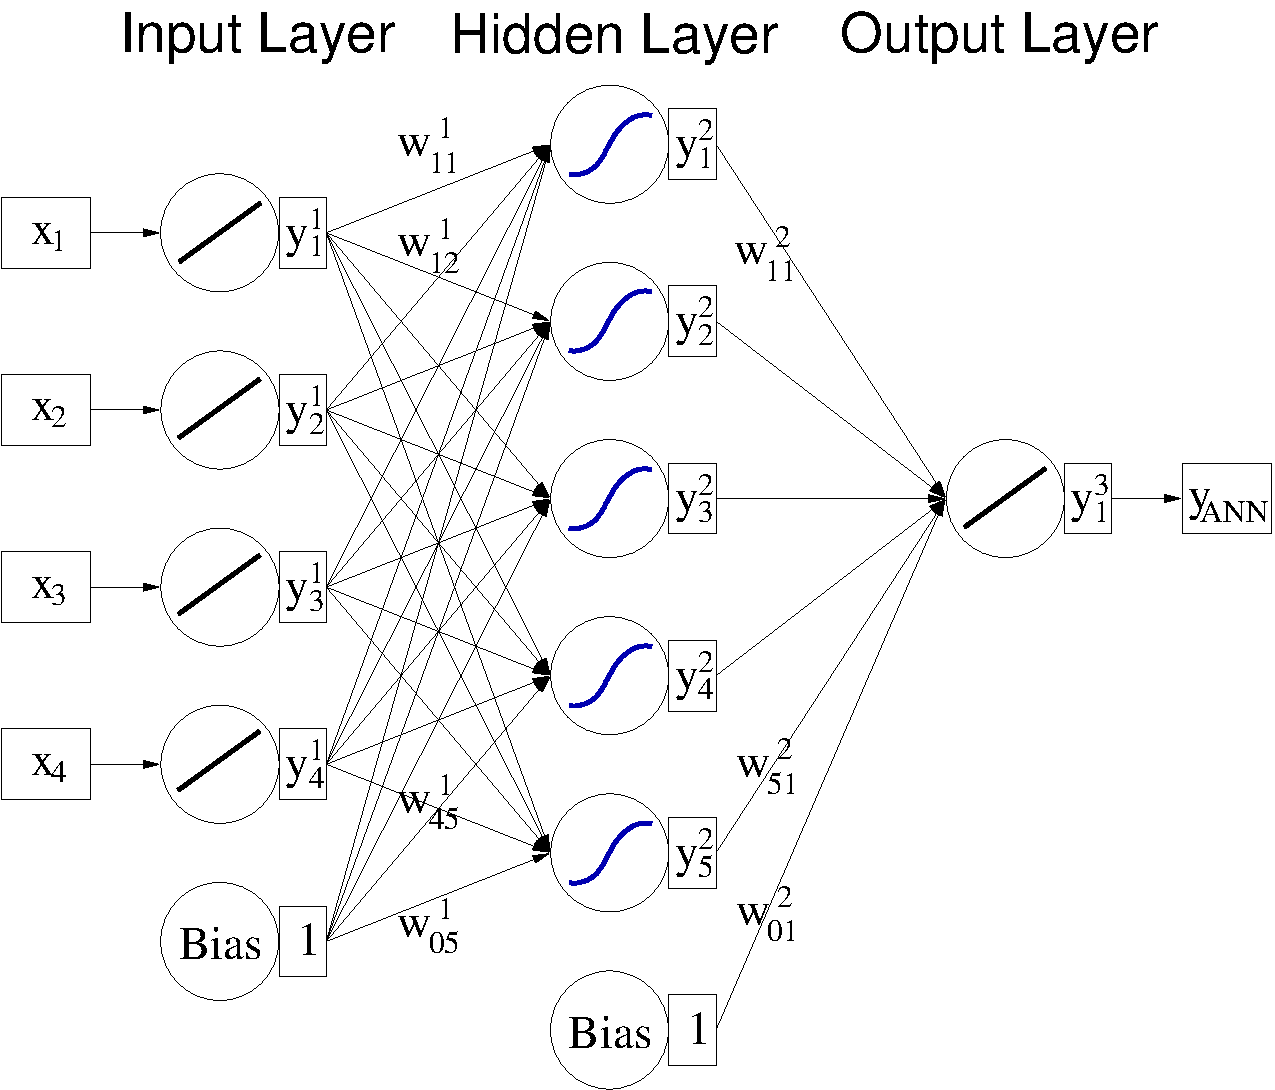
\includegraphics[width=0.62\textwidth]{plots/MLP}
  %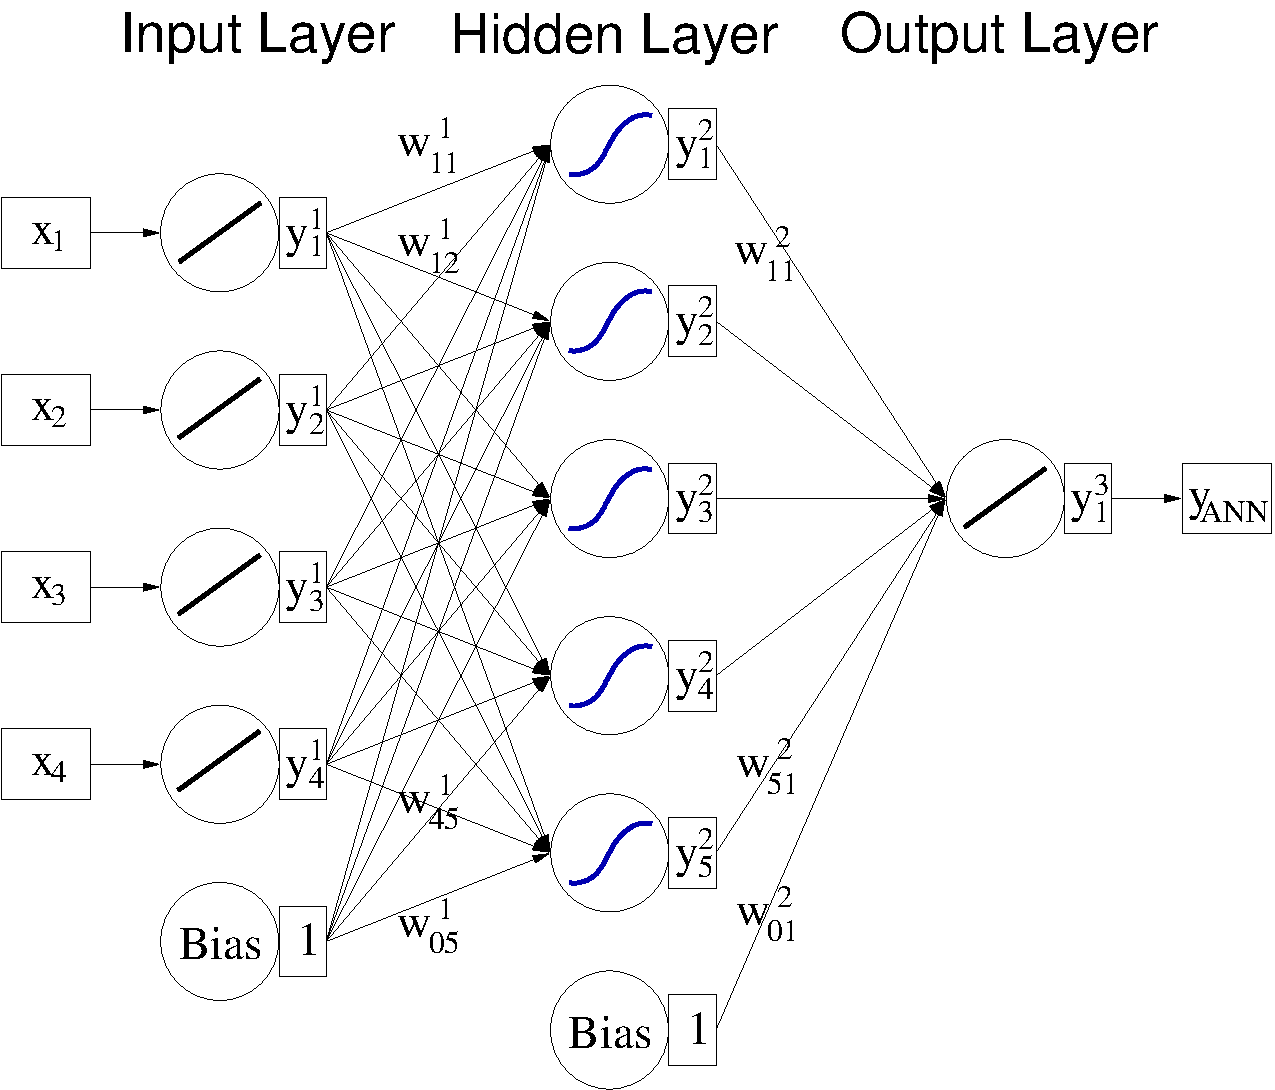
\epsfig{file=plots/MLP,width=0.62\textwidth}
  \caption[.]{Multilayer perceptron with one hidden layer.}
  \label{fig:mlp:nw}
\end{figure}
\begin{figure}[t]
  \centering
  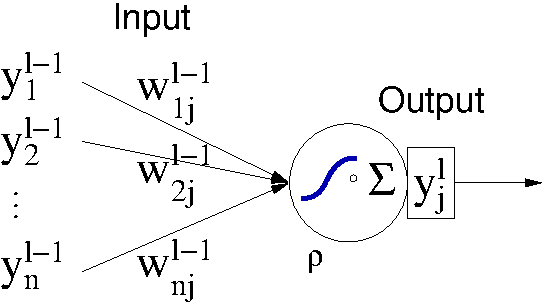
\includegraphics[width=.30\textwidth]{plots/MLP_SingleNode}
  %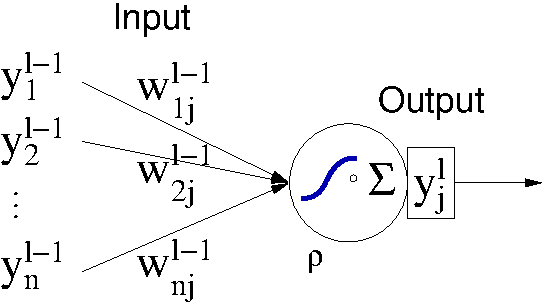
\epsfig{file=plots/MLP_SingleNode,width=.30\textwidth}
  \caption[.]{Single neuron $j$ in layer $\ell$ with $n$ input connections. The
    incoming connections carry a weight of $w_{ij}^{(l-1)}$.}
  \label{fig:mlp:node}
\end{figure}

\subsubsection*{Neuron response function}

The neuron response function $\rho$ maps the neuron input
$i_1,\dots,i_n$ onto the neuron output (Fig.~\ref{fig:mlp:node}).
Often it can be separated into a ${\cal R}^n\mapsto{\cal R}$
{\em synapse function} $\kappa$, and a ${\cal R}\mapsto{\cal R}$
{\em neuron activation function} $\alpha$, so that $\rho=\alpha\circ\kappa$.
The functions $\kappa$ and $\alpha$ can have the following forms:
\beq
  \label{eq:mlp:synfnc}
  \kappa:~(y_1^{(\ell)},..,y_n^{(\ell)}|w_{0j}^{(\ell)},..,w_{nj}^{(\ell)})\rightarrow
  \begin{cases}
    w_{0j}^{(\ell)}+\sum\limits_{i=1}^n y_{i}^{(\ell)} w_{ij}^{(\ell)}
         &\text{\em Sum},\\[0.3cm]
    w_{0j}^{(\ell)}+\sum\limits_{i=1}^n \left(y_{i}^{(\ell)} w_{ij}^{(\ell)}\right)^2
         &\text{\em Sum of squares},\\[0.3cm]
    w_{0j}^{(\ell)}+\sum\limits_{i=1}^n |y_{i}^{(\ell)} w_{ij}^{(\ell)}|
         &\text{\em Sum of absolutes},
  \end{cases}
\eeq
\beq
  \label{eq:mlp:actfnc}
  \alpha:~x\rightarrow
  \begin{cases}
    \ x                                   & \text{\em Linear},\\[0.2cm]
    \ \Dfrac{1}{1+e^{-kx}}                & \text{\em Sigmoid},\\[0.3cm]
    \ \Dfrac{e^{x}-e^{-x}}{e^{x}+e^{-x}}  & \text{\em Tanh},\\[0.3cm]
    \ e^{-x^2/2}                          & \text{\em Radial}.
  \end{cases}
\eeq

\subsubsection{Network architecture}
\label{sec:MLP:hiddenLayers}

The number of hidden layers in a network and the number of neurons in these
layers are configurable via the option \code{HiddenLayers}. For example the
configuration \code{"HiddenLayers=N-1,N+10,3"} creates a network with three
hidden layers, the first hidden layer with $\Nvar-1$ neurons, the second with
$\Nvar+10$ neurons, and the third with 3 neurons.

When building a network two rules should be kept in mind. The first is the
theorem by Weierstrass, which if applied to neural nets, ascertains
that for a multilayer perceptron a single
hidden layer is sufficient to approximate a given continuous correlation function
to any precision, provided that a sufficiently large number of neurons is used
in the hidden layer. If the available computing power and the size of the training
data sample suffice, one can increase the number of neurons in the hidden layer
until the optimal performance is reached.

It is likely that the same performance can be achieved with a
network of more than one hidden layer and a potentially much smaller
total number of hidden neurons. This would lead to a shorter training
time and a more robust network.

\subsubsection{Training of the neural network}

\subsubsection*{Back-propagation (BP)}

The most common algorithm for adjusting the weights that optimise the
classification performance of a neural network is the so-called
{\em back propagation.}\index{Back propagation}
It belongs to the family of supervised learning methods, where the desired output for
every input event is known. Back propagation is used by all neural networks in TMVA.
The output of a network (here for simplicity assumed to have a single hidden layer with
a Tanh activation function, and a linear activation function in the output layer) is
given by
\beq
  \label{eq:mlp:mvacalc}
  \yANN
  =
  \sum_{j=1}^{n_\text{h}} y_j^{(2)}w_{j1}^{(2)}
  =
  \sum_{j=1}^{n_\text{h}}\tanh\!\left(\sum_{i=1}^\Nvar x_iw_{ij}^{(1)}\right)\cdot w_{j1}^{(2)}\,,
\eeq
where \Nvar and $n_\text{h}$ are the number of neurons in the input
layer and in the hidden layer, respectively, $w^{(1)}_{ij}$ is the
weight between input-layer neuron $i$ and hidden-layer neuron $j$,
and $w^{(2)}_{j1}$ is the weight between the hidden-layer neuron $j$ and the
output neuron. A simple sum was used in Eq.~(\ref{eq:mlp:mvacalc})
for the synapse function $\kappa$.

During the learning process the network is supplied with $\Ntrain$ training
events ${\bf x}_a = (x_1,\dots,x_\Nvar)_a$, $a=1,\dots,\Ntrain$. For each
training event $a$ the neural network output $\yANNa$ is computed
and compared to the desired output $\hat y_a\in\{1,0\}$ (in classification 1 for signal
events and 0 for background events). An {\em error function} $E$, measuring
the agreement of the network response with the desired one, is defined by
\beq
  E({\bf x}_1,\dots,{\bf x}_{\Ntrain} | {\bf w})
  =
  \sum_{a=1}^{\Ntrain} E_a({\bf x}_a | {\bf w})
  =
  \sum_{a=1}^{\Ntrain} \frac12 \left(\yANNa - \hat y_{a}\right)^{2}\,,
\eeq
where ${\bf w}$ denotes the ensemble of adjustable weights in the network.
The set of weights that minimises the error function can be found using
the method of {\em steepest} or {\em gradient descent}, provided that the neuron
response function is differentiable with respect to the input weights. Starting
from a random set of weights ${\bf w}^{(\rho)}$ the weights are updated by moving a
small distance in ${\bf w}$-space into the direction $-{\boldsymbol\nabla}_{\bf w} E$
where $E$ decreases most rapidly
\beq
  \label{eq:mlp:weightIter}
  {\bf w}^{(\rho+1)} = {\bf w}^{(\rho)} - \eta {\boldsymbol\nabla}_{\bf w} E\,,
\eeq
where the positive number $\eta$ is the {\em learning rate}.

The weights connected with the output layer are updated by
\beq
\label{eq:mlp:ouputupdate}
  \Delta w_{j1}^{(2)}
  =
  -\eta\sum_{a=1}^{\Ntrain} \frac{\partial E_a}{\partial w_{j1}^{(2)}}
  =
  -\eta\sum_{a=1}^{\Ntrain}\left(\yANNa - \hat y_{a}\right) y^{(2)}_{j,a}\,,
\eeq
and the weights connected with the hidden layers are updated by
\beq
\label{eq:mlp:hiddenupdate}
  \Delta w_{ij}^{(1)}
  =
  -\eta\sum_{a=1}^{\Ntrain} \frac{\partial E_a}{\partial w_{ij}^{(1)}}
  =
  -\eta\sum_{a=1}^{\Ntrain} \left(\yANNa - \hat y_{a}\right)
                                   y^{(2)}_{j,a}(1-y^{(2)}_{j,a}) w_{j1}^{(2)} x_{i,a}\,,
\eeq
where we have used $\tanh^\prime x = \tanh x(1-\tanh x)$. This method of training the
network is denoted {\em bulk learning}, since the sum of errors of all training
events is used to update the weights. An alternative choice is the so-called
{\em online learning}, where the update of the weights occurs at each event.
The weight updates are obtained from Eqs.~(\ref{eq:mlp:ouputupdate}) and
(\ref{eq:mlp:hiddenupdate}) by removing the event summations.
In this case it is important to use a well randomised training sample.
Online learning is the learning method implemented in TMVA.

\subsubsection*{BFGS}

The Broyden-Fletcher-Goldfarb-Shannon (BFGS)\index{BFGS} method~\cite{BFGS} differs from
back propagation by the use of second derivatives of the error function to
adapt the synapse weight by an algorithm which is composed of four main steps.
\begin{enumerate}

\item Two vectors, $D$ and $Y$ are calculated. The vector of weight changes
      $D$ represents the evolution between one iteration of the algorithm $(k-1)$
      to the next $(k)$. Each synapse weight corresponds to one element of the
      vector. The vector $Y$ is the vector of gradient errors.
      \beqn
        D_{i}^{(k)} &=& w_i^{(k)} - w_i^{(k-1)}\:,  \\
        Y_{i}^{(k)} &=& g_i^{(k)} - g_i^{(k-1)}\:,
      \eeqn
      where $i$ is the synapse index, $g_i$ is the $i$-th synapse gradient,\footnote
      {
         The synapse gradient is estimated in the same way as in the BP method
         (with initial gradient and weights set to zero).
      }
      $w_i$ is the weight of the $i$-th synapse, and $k$ denotes the iteration counter.

\item Approximate the inverse of the Hessian matrix, \IHessian, at iteration $k$ by
      \beq
        \IHessiank = \frac{D\cdot D^{T}\cdot (1+Y^{T}\cdot \IHessiankmone\cdot Y)}{Y^{T}\cdot D}
                       - D\cdot Y^{T}\cdot H + H\cdot Y\cdot D^{T} + \IHessiankmone\:,
      \eeq
      where superscripts $(k)$ are implicit for $D$ and $Y$.

\item Estimate the vector of weight changes by
      \beq
        D^{(k)} = -\IHessiank\cdot Y^{(k)}\:.
      \eeq

\item Compute a new vector of weights by applying a {\em line search} algorithm.
In the line search the error function is locally approximated
by a parabola. The algorithm evaluates the second derivatives and
determines the point where the minimum of the parabola
is expected. The total error is evaluated for this point. The algorithm then
evaluates points along the line defined by the direction of the gradient
in weights space to find the absolute minimum. The weights at the
minimum are used for the next iteration. The learning rate can be set
With the option \code{Tau}. The learning
parameter, which defines by how much the weights are changed in one epoch
along the line where the minimum is suspected, is multiplied with the
 learning rate as long as the training error of the
neural net with the changed weights is below the one with unchanged weights.
If the training error of the changed neural net were already larger
for the initial learning parameter, it is divided by the learning rate
until the training error becomes smaller.
The iterative and approximate calculation of $\IHessiank$ turns less
accurate with an increasing number of iterations. The
matrix is therefore reset to the unit matrix every \code{ResetStep} steps.
\end{enumerate}

The advantage of the BFGS method compared to BG is the smaller number of
iterations. However, because the computing time for one iteration is
proportional to the squared number of synapses, large networks are
particularly penalised.

\subsubsection{Variable ranking}
\label{sec:ann:ranking}

The MLP neural network implements a variable ranking that uses the sum of the
weights-squared of the connections between the variable's neuron in the input
layer and the first hidden layer. The importance $I_i$ of the input variable
$i$ is given by
\beq
  \label{eq:mlp:ranking}
  I_i = \overline x_i^2 \sum_{j=1}^{n_\text{h}} \left(w^{(1)}_{ij}\right)^2, \qquad i=1,\dots,\Nvar\,,
\eeq
where $\overline x_{i}$ is the sample mean of input variable $i$.

\subsubsection{Bayesian extension of the MLP}
\label{sec:ann:bayes}
Achieiving a good test performance with MLP is a tradeoff between using a network architecture that is flexible enough to allow for the modelling of complex functions and the avoidance of overtraining. Avoiding overtraining by limiting the flexibility of the network in the first place by keeping the number of hidden units/layers small is a very rigid approach which will typically hurt the performance of the neural network. The Bayesian extension of MLP offers a means to allow for more complex network architectures while at the same time regularizing the model complexity adaptively to avoid unwanted overfitting effects. The price to pay is an increase in computation time. The extension is enabled with the option \code{UseRegulator} and should typically be used in difficult setting where the problem calls for a network architecture with many hidden units and/or several layers.
Enabling the Bayesian extension of the MLP will add an additional term to the network error function $E(\bf w)$ (which is equivalent to minus the log-likelihood of the training data given the network model):
\beq
  \label{eq:mlp:penalty}
	\tilde{E}(\bf w) = E(\bf w) + \alpha\bf |w|^2
\eeq
The penalty term is proportional to the squared norm of the weight ensemble $\bf w$ of the network and effectively penalizes large weights which results in a reduced model complexity. The metaparameter $\alpha$ controls the amount of regularization applied and thus ultimatively controls the level of model complexity the network can exhibit. This is called a Bayesian extension since it is equivalent to introducing a Gaussian prior for the network weights, whose width is controlled by the parameter $\alpha$. Since choosing $\alpha$ manually would only shift the problem of picking the correct network complexity to picking the right $\alpha$, TMVA automatically infers the best value of $\alpha$ from the training data by doing a complexity analysis based on the so-called evidence approximation. The user can therefore choose to train a large network which will then automatically be regularized to a degree that optimally fits the data.

\subsubsection{Performance}
\label{sec:ann:perf}

In the tests we have carried out so far, the MLP and ROOT networks performed equally well,
however with a clear speed advantage for the MLP. The Clermont-Ferrand neural net
exhibited worse classification performance in these tests, which is partly due to the slow
convergence of its training (at least 10k training cycles are required to achieve
approximately competitive results).


%%% Local Variables:
%%% mode: latex
%%% TeX-master: "TMVAUsersGuide"
%%% End:
